\section{Server}

The server is the central component of \snowman{} and generally consists of:

\begin{itemize}
  \item Central rule storage
  \item Web-interface for user interaction
  \item Update-module to get updates from rule-sources
  \item RPC-interface to communicate with the clients
\end{itemize}

The central storage of rules would be a normal relation database. As we have
decided to use Django as our framework, we have a great flexibility to which
database we actually use. In the current version of \django{} (1.6) we might use
MySQL, PostgreSQL, SQLite or Oracle.

For the RPC-Interface, we have decided to use
XML-RPC. This is a very simple protocol using XML over HTTP to transfer 
requests and data to and from the server. To be able to keep an aspect of
privacy, we encrypt the raw HTTP stream using SSL. 

\subsection{Architecture}

The server architecture follows the layered
approach of MVC (figure \ref{fig:server_architecture}).

\begin{figure}[h]
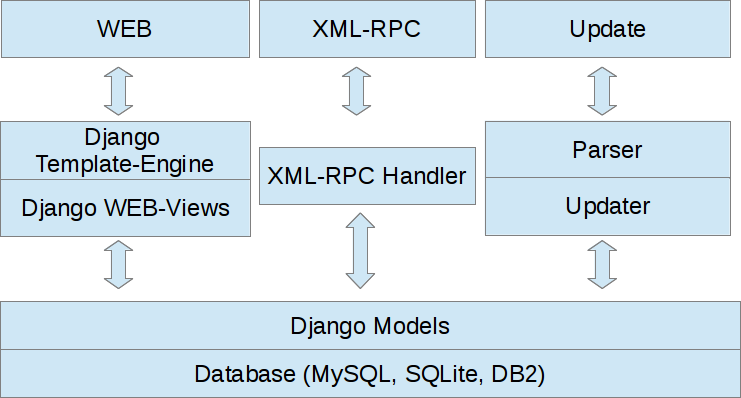
\includegraphics[width=130mm]{./img/Server-MVC.png}
\caption{Server Architecture}
\label{fig:server_architecture}
\end{figure}

The web-interface uses pure Django logic. The HTML visible in the users
browser is generated by the Django template-engine, which recieves its data
from the views created by using ordinary pyhton code.

The XML-RPC server uses a handler which is administering the connections from
the sensors, and exposing the relevant methods to allow the sensors do a
synchronization.

The update is unpacking and preparing the update-files for parsing. It then
handles the files to the parser. The parser is then handling the different
parametres to the Updater, which in turn saves them to the database in an
efficient manner.

Finally, common for all the interfaces is the Django Models. We use the
database-abstractionlayer from Django for mapping the lines of a
relational-database to django objects. This is the part that lets us write code
once, and still be able to use several different database-engines.

\subsection{Database}

As the database of the server is quite complex, we have divided the drawings, so
that we have one drawing per module.

\subsubsection{Core}

The core database-architecture used for storing the rules is as following:

\begin{figure}[h]
	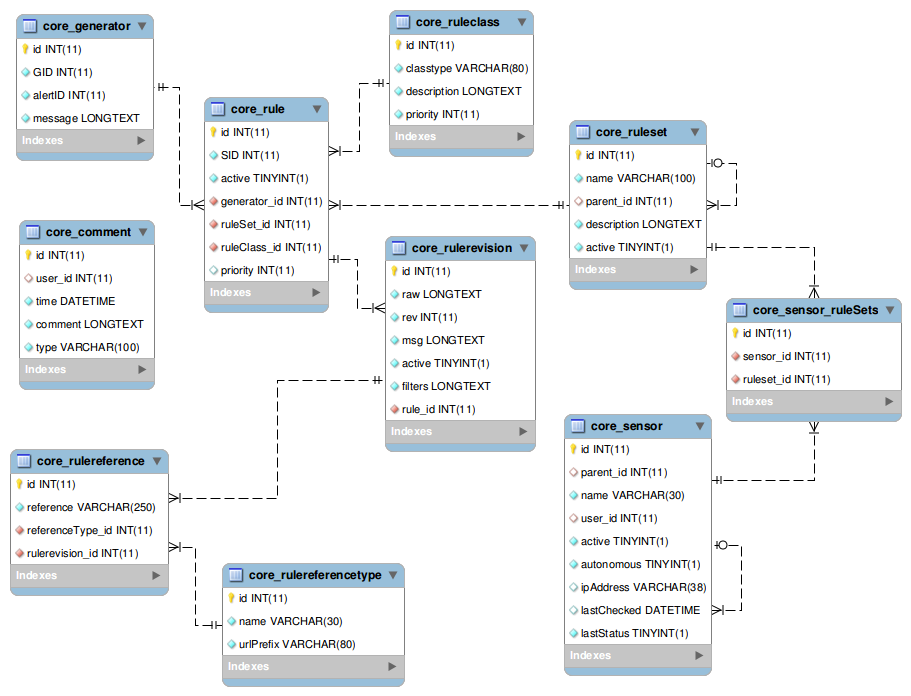
\includegraphics[width=127mm]{./img/Server-DB-Core.png}
	\caption{Core server-database}
	\label{fig:server_database_core}
\end{figure}

The most central part of our system is the representation of a Rule. A single
Rule might have several revisions, as we might want to keep some history when
they get updated. Each revision have its own set of references attached.

A single rule also have a lot of other properties which it might share with
other rules. A generator, a classification and a ruleset are examples of such.

Finally, the rules are placed onto a sensor by attaching ruleSets to the
sensors.

\subsubsection{Tuning}

In addition to storing the raw rules, we would like to be able to store
tuning-parametres on the rules. As sensors might have different
tuning-parametres, we cannot add the tuning directly to the rules. We rather add
the tuning to its own module:

\begin{figure}[h]
	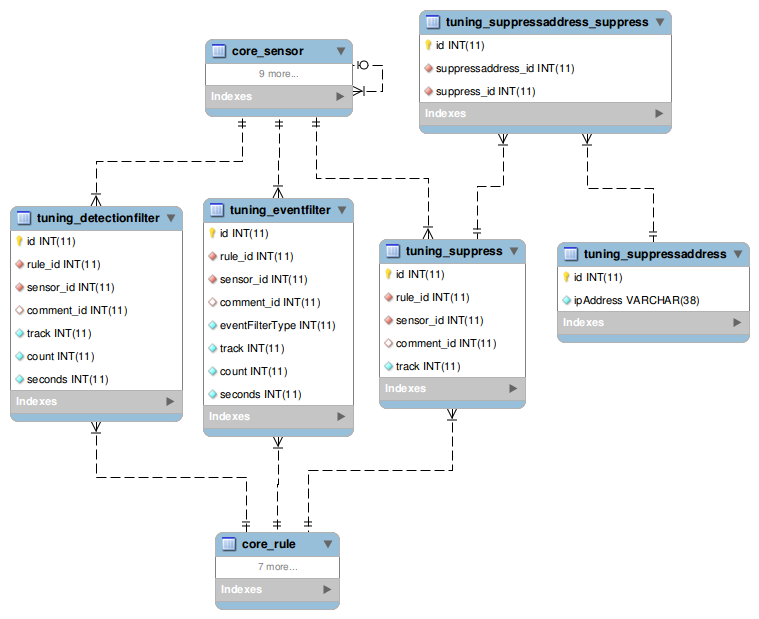
\includegraphics[width=127mm]{./img/Server-DB-Tuning.png}
	\caption{Tuning server-database}
	\label{fig:server_database_tuning}
\end{figure}

Both filters, and the suppresses is connected to a Rule and a Sensor. This way
we let the user spesify filters for the individual sensors if that is desired.
If a sensor does not have a filter applied, but any parent of the sensor have
one, the closest parent's filter will be applied.

\subsubsection{Update}

When rules are inserted to the database, we would like to have some traceability
to be able to determine from where a rule have entered our system. To be able to
do this, we have the update-module:

\begin{figure}[h]
	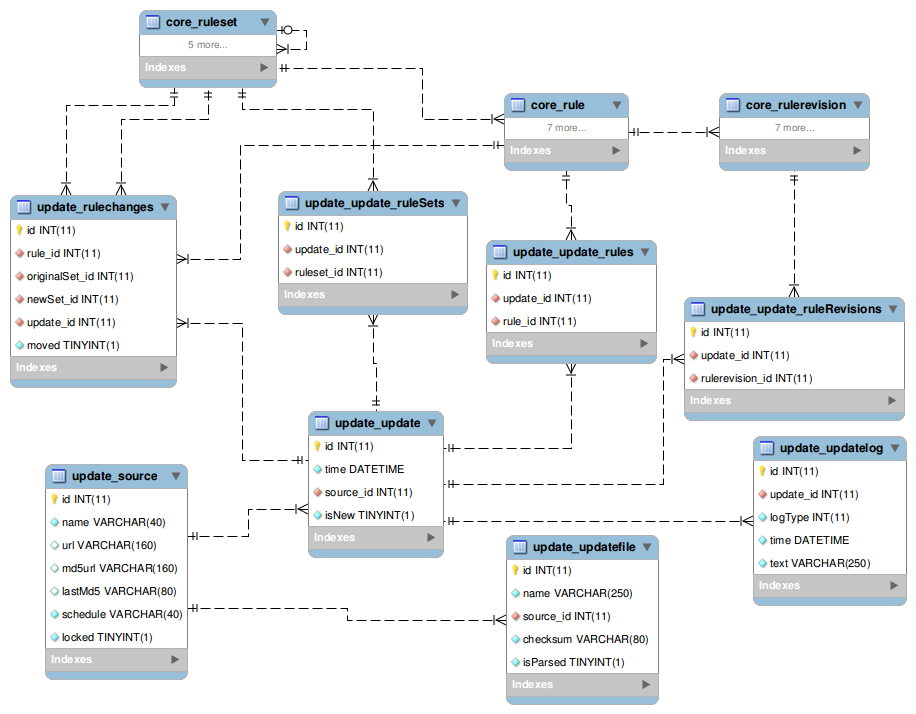
\includegraphics[width=127mm]{./img/Server-DB-Update.png}
	\caption{Update server-database}
	\label{fig:server_database_update}
\end{figure}

The structure of the database to update would let us store the update-sources,
and add a update-object for each update ran from a given source. These update
objects can in turn have a relation to rules, rulesets and rulerevisions, so
that we can track what changes for each update.